\begin{flushright} {\tiny {\color{gray} mccriterion.tex}} \end{flushright}
%~~~~~~~~~~~~~~~~~~~~~~~~~~~~~~~~~~~~~~~~~~~~~~~~~~~~~~~~~~~~~~~~~~~~~~~~~~~~~~~~~~~~~~~~~~~~~~~~~~

Mohr-Coulomb theory is a model describing the response of a material such as rubble piles or concrete to shear stress as well as normal stress. 
Most of the classical engineering materials somehow follow this rule in at least a portion of their shear failure envelope. In geology it is used to define shear strength of soils at different effective stresses \cite{hand69}.

In structural engineering it is used to determine failure load as well as the angle of fracture of a displacement fracture in concrete and similar materials. Coulomb's friction hypothesis is used to determine the combination of shear and normal stress that will cause a fracture of the material. Mohr's circle is used to determine the principal stresses that will produce this combination of shear and normal stress, and the angle of the plane in which this will occur. According to the principle of normality, the stress introduced at failure will be perpendicular to the line describing the fracture condition.

%It can be shown that a material failing according to Coulomb's friction hypothesis will show the displacement introduced at failure forming an angle to the line of fracture equal to the angle of friction. This makes the strength of the material determinable by comparing the external mechanical work introduced by the displacement and the external load with the internal mechanical work introduced by the strain and stress at the line of failure. By conservation of energy the sum of these must be zero and this will make it possible to calculate the failure load of the construction.

\begin{center}
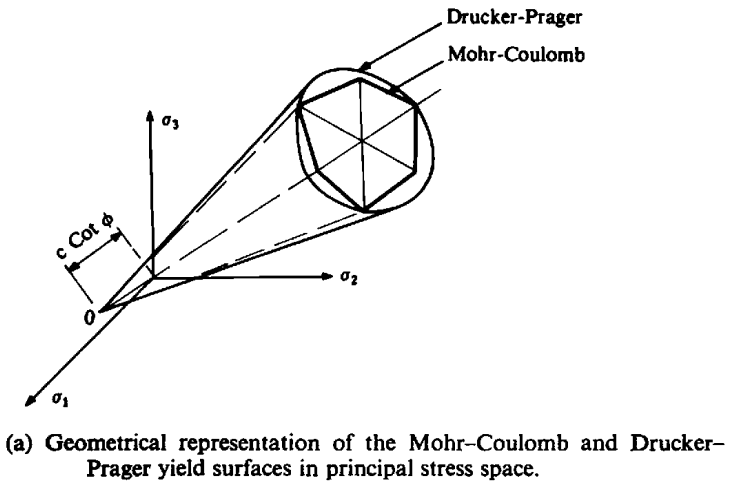
\includegraphics[width=6cm]{images/rheology/owenhinton5}\\
{\captionfont Taken from \textcite{owhi}.}
\end{center}

The Mohr-Coulomb failure criterion represents the linear envelope that is obtained 
from a plot of the shear strength of a material 
versus the applied normal stress. This relation is expressed as (Owen \& Hinton book \cite[p219]{owhi})
%\[
%\tau = c- \sigma~\tan(\phi) 
%\]

%Compression is assumed to be positive in the following discussion. If compression is assumed to be negative then $\sigma$ should be replaced with $-\sigma$.

%If $\phi=0$, the Mohr-Coulomb criterion reduces to the Tresca criterion. On the other hand, if $\phi = 90^\circ$ the Mohr-Coulomb model is equivalent to the Rankine model. Higher values of $\phi$ are not allowed.

\begin{equation}
\tau_m = -\sigma_m \sin \phi + c \cos \phi  \label{eq:mccrit}
\end{equation}
where $\tau_m$ is the magnitude of the shear stress, 
$\sigma_m$ is the normal stress, $c$ is the intercept of the failure envelope with the $\tau$ axis, 
and $\phi$ is the slope of the failure envelope.
The minus sign in the above equation is for the case where compression is assumed to be 
negative\footnote{\url{https://en.wikipedia.org/wiki/Mohr-Coulomb_theory}}.
The quantity $c$ is often called the cohesion and the angle $\phi$ is called the angle of internal friction.
 
We have  
\[
\tau_m=\frac{\sigma_1-\sigma_3}{2}
\qquad
\qquad
\sigma_m = \frac{\sigma_1+\sigma_3}{2}
\]
with $\sigma_1$ is the maximum principal stress and $\sigma_3$ is the minimum principal stress, or
%\[
%\sigma_1-\sigma_3 = - ( \sigma_1+\sigma_3) \sin \phi + 2c \cos \phi
%\]
%\[
%\sigma_1-\sigma_3 = 2 c \cos \phi - (\sigma_1+\sigma_3) \sin\phi
%\]
\begin{equation}
\cfrac{\sigma_1-\sigma_3}{2} = -\cfrac{\sigma_1+\sigma_3}{2}~\sin\phi +c\; \cos\phi 
\end{equation}
Using Eqs.~\eqref{eq:sig13a} and \eqref{eq:sig13b} 
for $(\sigma_1 - \sigma_3 )/2$ and $(\sigma_1 + \sigma_3 )/2$ we get\footnote{This is 
Eq.~(7.16) of \textcite{owhi}}:
\begin{eqnarray}
&& \frac{\sigma_1 - \sigma_3}{2} = -\frac{\sigma_1 + \sigma_3}{2} \sin \phi  + c \cos \phi \nn\\
&\Rightarrow&
\sqrt{  {\cal I}_2({\bm \tau}) } \cos \theta = -\left(\frac{1}{3}{\cal I}_1({\bm \sigma}) - \sqrt{  {\cal I}_2({\bm \tau})} \frac{1}{\sqrt{3}} \sin \theta \right) \sin \phi 
+ c \cos \phi \nn\\
&\Rightarrow&
\frac{1}{3} {\cal I}_1({\bm \sigma}) \sin \phi  
+ \sqrt{  {\cal I}_2({\bm \tau}) } \left( \cos \theta - \frac{1}{\sqrt{3}} \sin \theta  \sin \phi \right) - c \cos \phi = 0 \nn
\end{eqnarray}

\begin{mdframed}[backgroundcolor=blue!5]
\begin{equation}
F^{\text{\tiny MC}}=\frac{1}{3} {\cal I}_1({\bm \sigma}) \sin \phi  + 
\sqrt{  {\cal I}_2({\bm \tau})  } \left( \cos \theta - \frac{1}{\sqrt{3}} \sin \theta  \sin \phi \right) - c \cos \phi
\label{eq:mcF} 
\end{equation}
\end{mdframed}
This formula (without the cohesion) is used in \textcite{will92}.
Since $p=-\frac{1}{3} {\cal I}_1({\bm \sigma})$, we also have:
%\begin{equation}
%F^{\text{\tiny MC}}= -p \sin \phi  + 
%\sqrt{ {\cal I}_2({\bm \tau})  } \left( \cos \theta - \frac{1}{\sqrt{3}} \sin \theta  \sin \phi \right) - c \cos \phi 
%\end{equation}
%or, 
\begin{mdframed}[backgroundcolor=blue!5]
\begin{equation}
F^{\text{\tiny MC}}=
\sqrt{  {\cal I}_2({\bm \tau})  } \left( \cos \theta - \frac{1}{\sqrt{3}} \sin \theta  \sin \phi \right) - (p \sin\phi + c \cos \phi)
\end{equation}
\end{mdframed}

\begin{remark}
The expression for $F$ in the Mohr-Coulomb case in Zienkiewicz \& Cormeau (1974) \cite{zico74} 
contains errors which are later corrected in \textcite[p102]{book_zitf}. 
\end{remark}

\Literature: this criterion is also used in computer graphics animation \cite{zhbr05}

\todo{when $\phi=0$ we should recover Tresca but factor 2 is wrong ?}



\vspace{.5cm}

We now look into the derivatives of the Drucker-Prager plastic potential $Q^{\text{\tiny MC}}(\bm\sigma)$.
We have
\[
Q^{\text{\tiny MC}}=
\frac{1}{3} {\cal I}_1({\bm \sigma}) \sin \phi  + 
\sqrt{  {\cal I}_2({\bm \tau})  } \left(\cos\theta_{\rm L}(\bm\tau)-\frac{1}{\sqrt{3}} 
\sin\theta_{\rm L} (\bm\tau) \sin\phi \right) -c \cos \phi
\]
Then
\begin{eqnarray}
\frac{\partial Q^{\text{\tiny MC}}  }{\partial {\cal I}_1(\bm\sigma)} &=& \frac13 \sin\phi \\
\frac{\partial Q^{\text{\tiny MC}}  }{\partial \sqrt {{\cal I}_2(\bm\tau)}}
&=&  
\cos \theta_{\rm L} - \frac{1}{\sqrt{3}} \sin \theta_{\rm L}  \sin \phi  
+  \sqrt{  {\cal I}_2({\bm \tau})  } 
\left(-\sin \theta_{\rm L} - \frac{1}{\sqrt{3}} \cos \theta_{\rm L}  \sin \phi \right) 
\frac{\partial \theta_{\rm L}}{\partial \sqrt {{\cal I}_2(\bm\tau)}   } \nn \\
&=&  
\cos \theta_{\rm L} - \frac{1}{\sqrt{3}} \sin \theta_{\rm L}  \sin \phi  
+  \sqrt{  {\cal I}_2({\bm \tau})  } 
\left(-\sin \theta_{\rm L} - \frac{1}{\sqrt{3}} \cos \theta_{\rm L}  \sin \phi \right) 
\frac{\partial \theta_{\rm L}}{\partial  {{\cal I}_2(\bm\tau)}   }  
\frac{\partial   {{\cal I}_2(\bm\tau)}     }{\partial \sqrt {{\cal I}_2(\bm\tau)}   }  \nn\\
&=&  
\cos \theta_{\rm L} - \frac{1}{\sqrt{3}} \sin \theta_{\rm L}  \sin \phi  
+  \sqrt{  {\cal I}_2({\bm \tau})  } 
\left(-\sin \theta_{\rm L} - \frac{1}{\sqrt{3}} \cos \theta_{\rm L}  \sin \phi \right) 
\left(
-\frac12 \tan 3\theta_{\rm L} \frac{1}{ {\cal I}_2(\bm\tau)} 
\right)
2 \sqrt {{\cal I}_2(\bm\tau)} \nn \\
&=&  
\cos \theta_{\rm L} - \frac{1}{\sqrt{3}} \sin \theta_{\rm L}  \sin \phi  
+  
\left(\sin \theta_{\rm L} + \frac{1}{\sqrt{3}}\cos\theta_{\rm L}\sin\phi\right) \tan 3\theta_{\rm L} \nn\\
&=&  
\cos \theta_{\rm L}
\left[
1 - \frac{1}{\sqrt{3}} \tan \theta_{\rm L}  \sin \phi  
+  
\left(\tan \theta_{\rm L} + \frac{1}{\sqrt{3}}   \sin \phi \right)  \tan 3\theta_{\rm L} 
\right] \nn\\
&=&
\cos \theta_{\rm L}
\left[
(1 +  \tan \theta_{\rm L}   \tan 3\theta_{\rm L})
+\frac{1}{\sqrt{3}} \sin\phi
( \tan 3\theta_{\rm L} - \tan\theta_{\rm L})
\right]
\\ 
\frac{\partial Q^{\text{\tiny MC}} }{\partial \theta_{\rm L}(\bm\tau)} 
&=&  
\sqrt{{\cal I}_2(\bm \tau)} (-\sin\theta_{\rm L}-\frac{1}{\sqrt{3}} \cos\theta_{\rm L} \sin\phi )\nn\\
&=&  
-\frac{1}{\sqrt{3}} \sqrt{{\cal I}_2(\bm \tau)} (\sqrt{3} \sin\theta_{\rm L}+\cos\theta_{\rm L} \sin\phi )
\end{eqnarray}
so
\begin{eqnarray}
C_1^{\text{\tiny MC}} &=& \frac13 \sin\phi  \\ 
C_2^{\text{\tiny MC}} 
&=& 
\frac{1}{2 \sqrt{ {\cal I}_2(\bm\tau)}   }   
\left( \frac{\partial Q}{\partial \sqrt{{\cal I}_2(\bm\tau)}} 
- \frac{\tan 3\theta_{\rm L}}{\sqrt {{\cal I}_2(\bm\tau)}}
\frac{\partial Q}{\partial \theta_{\rm L}(\bm\tau)}  
\right) \nn\\
&=& 
\frac{1}{2 \sqrt{ {\cal I}_2(\bm\tau)}   }   
\left( \cos \theta_{\rm L} \left[
(1 +  \tan \theta_{\rm L}   \tan 3\theta_{\rm L})
+\frac{1}{\sqrt{3}} \sin\phi ( \tan 3\theta_{\rm L} - \tan\theta_{\rm L}) \right]
+ \frac{\tan 3\theta_{\rm L}}{\sqrt {{\cal I}_2(\bm\tau)}}
\frac{1}{\sqrt{3}} \sqrt{{\cal I}_2(\bm \tau)} (\sqrt{3} \sin\theta_{\rm L}+\cos\theta_{\rm L} \sin\phi )
\right) \nn\\
&=& 
\frac{1}{2 \sqrt{ {\cal I}_2(\bm\tau)}   }   
\left( \cos \theta_{\rm L}
\left[ (1 +  \tan \theta_{\rm L}   \tan 3\theta_{\rm L})
+\frac{1}{\sqrt{3}} \sin\phi
( \tan 3\theta_{\rm L} - \tan\theta_{\rm L}) \right]
+ \tan 3\theta_{\rm L}  ( \sin\theta_{\rm L}+\frac{1}{\sqrt{3}}\cos\theta_{\rm L} \sin\phi )
\right) \nn\\
&=& 
\frac{1}{2 \sqrt{ {\cal I}_2(\bm\tau)}   }   
\left( \cos \theta_{\rm L} \left[
(1 +  \tan \theta_{\rm L}   \tan 3\theta_{\rm L})
+\frac{1}{\sqrt{3}} \sin\phi
( \tan 3\theta_{\rm L} - \tan\theta_{\rm L})
+ \tan 3\theta_{\rm L}   ( \tan\theta_{\rm L}+\frac{1}{\sqrt{3}} \sin\phi )
\right] \right) \nn\\
&=& 
\frac{1}{2 \sqrt{ {\cal I}_2(\bm\tau)}   }   
\cos \theta_{\rm L} \left[
(1 +  2\tan \theta_{\rm L}   \tan 3\theta_{\rm L})
+\frac{1}{\sqrt{3}} \sin\phi ( 2\tan 3\theta_{\rm L} - \tan\theta_{\rm L})
\right] \nn\\
C_3^{\text{\tiny MC}} 
&=&  - \frac{\sqrt{3}}{2\cos 3\theta_{\rm L}}
\frac{1}{{\cal I}_2(\bm\tau)^{3/2}} 
\frac{\partial Q}{\partial \theta_{\rm L}(\bm\tau)} \nn\\ 
&=&  - \frac{\sqrt{3}}{2\cos 3\theta_{\rm L}}
\frac{1}{{\cal I}_2(\bm\tau)^{3/2}} 
\left[-\frac{1}{\sqrt{3}} \sqrt{{\cal I}_2(\bm \tau)} (\sqrt{3} \sin\theta_{\rm L}+\cos\theta_{\rm L} 
\sin\phi ) \right]  \nn\\
&=&  \frac{\sqrt{3}\sin\theta_{\rm L} +  \sin \phi \cos \theta_{\rm L}}
{2 {\cal I}_2({\bm \tau}) \cos 3\theta_{\rm L}}
\end{eqnarray}










%\newpage
%\paragraph{two-dimensional space}

%The principal stress values are given by
%\[
%\sigma_{1,3} = \frac{\sigma_{xx}+\sigma_{yy}}{2} \pm \sqrt{ \frac{1}{4}(\sigma_{xx}-\sigma_{yy})^2 + \sigma_{xy}^2  }
%= \frac{J_1}{2} \pm \sqrt{ J_2'}
%\]
%so
%\[
%\frac{\sigma_1-\sigma_3}{2} = \frac{\sqrt{J_2}- - \sqrt{J_2}}{2} = \sqrt{J_2}
%\]
%\[
%\frac{\sigma_1+\sigma_3}{2} =  \frac{J_1}{2} 
%\]
%and then
%\[
%\sqrt{J_2} = - \frac{J_1}{2} \sin\phi + c\cos\phi 
%\]
%The Mohr-Coulomb criterion simply writes:
%
%\begin{mdframed}[backgroundcolor=blue!5]
%\begin{equation}
%F^{MC,2D}=  \frac{J_1}{2} \sin \phi + \sqrt{J_2} - c  \cos \phi  \label{mc2Dcriterion}
%\end{equation}
%\end{mdframed}

%%%%%%%%%%%%%%%%%%%%%%%%%%%%%%%%%%%%
%\paragraph{three-dimensional space}
%The Haigh-Westergaard invariants are related to the principal stresses by
%\begin{eqnarray}
%\sigma_1 &=& \cfrac{1}{\sqrt{3}}~\xi + \sqrt{\cfrac{2}{3}}~\rho~\cos\theta  \nonumber\\
%\sigma_3 &=& \cfrac{1}{\sqrt{3}}~\xi + \sqrt{\cfrac{2}{3}}~\rho~\cos\left(\theta+\cfrac{2\pi}{3}\right) \nonumber
%\end{eqnarray}
%Plugging into the expression for the Mohr-Coulomb yield function gives us
%\[
% -\sqrt{2}~\xi~\sin\phi + \rho[\cos\theta - \cos(\theta+2\pi/3)] - \rho\sin\phi[\cos\theta+\cos(\theta+2\pi/3)] = \sqrt{6}~c~\cos\phi 
%\]
%Using trigonometric identities for the sum and difference of cosines and rearrangement gives us the expression of the Mohr-Coulomb yield function in terms of $\xi$, $\rho$ and $\theta$:
%\[
%\left[\sqrt{3}~\sin\left(\theta+\cfrac{\pi}{3}\right) - \sin\phi\cos\left(\theta+\cfrac{\pi}{3}\right)\right]\rho - \sqrt{2}\sin(\phi)\xi = \sqrt{6} c \cos\phi 
%\]
%Alternatively, in terms of the invariants $p$,$q$,$r$ we can write
%\[
%\left[\cfrac{1}{\sqrt{3}~\cos\phi}~\sin\left(\theta+\cfrac{\pi}{3}\right) - \cfrac{1}{3}\tan\phi~\cos\left(\theta+\cfrac{\pi}{3}\right)\right]q - p~\tan\phi = c 
%\]

\newpage
